\documentclass[a4paper, 11pt]{article}

\setcounter{tocdepth}{3}
\setcounter{secnumdepth}{3}

\usepackage{comment} % enables the use of multi-line comments (\ifx \fi) 
\usepackage{lipsum} %This package just generates Lorem Ipsum filler text. 
\usepackage{fullpage} % changes the margin
\usepackage[utf8]{inputenc}
\usepackage{gensymb}
\usepackage{graphicx}
\usepackage{booktabs}% http://ctan.org/pkg/booktabs
\usepackage{makecell}
\usepackage{tabularx}
\usepackage[table]{xcolor}
\usepackage{array}
\usepackage{wrapfig}
\usepackage{subcaption}
\usepackage{csquotes}
\usepackage{lscape}
\usepackage{afterpage}
\usepackage{geometry}
\usepackage{listingsutf8}
\usepackage{chngcntr}
\usepackage{multicol}
\usepackage{xcolor}
\usepackage{pifont}
\usepackage{outlines}
\usepackage{booktabs}% http://ctan.org/pkg/booktabs
\usepackage{amsmath}



\counterwithin{figure}{section}

\AtBeginDocument{\counterwithin{lstlisting}{section}}

\geometry{a4paper, margin=1in}

\renewcommand*{\thead}[1]{\bfseries #1}

\newcommand{\code}[1]{\texttt{#1}}
\newcommand \tabitem{\makebox[1em][r]{\textbullet~}}

\DeclareMathSizes{12}{30}{16}{12}

\definecolor{lightgray}{rgb}{.9,.9,.9}
\definecolor{darkgray}{rgb}{.4,.4,.4}
\definecolor{purple}{rgb}{0.65, 0.12, 0.82}
\definecolor{darkgreen}{rgb}{0.05,0.56,0.06}


\lstset{frame=tlrb,
    language=python,
    captionpos=b,
    aboveskip=3mm,
    belowskip=3mm,
    showstringspaces=false,
    columns=flexible,
    basicstyle={\small\ttfamily},
    numbers=left,
    numberstyle=\tiny\color{gray},
    keywordstyle=\color{blue},
    commentstyle=\color{violet},
    stringstyle=\color{darkgreen},
    breaklines=true,
    breakatwhitespace=true,
    tabsize=3,
    literate=%
    {Ö}{{\"O}}1
    {Ä}{{\"A}}1
    {Ü}{{\"U}}1
    {ß}{{\ss}}1
    {ü}{{\"u}}1
    {ä}{{\"a}}1
    {ö}{{\"o}}1
}


\begin{document}

\newgeometry{top=0in, bottom=0in}
\title{Machine Learning FS2019}
\author{Alex Neher}
\maketitle

\tableofcontents

\newpage
\graphicspath{{./Pictures/}}

\restoregeometry

\section{Introduction}

There are two popular definitions of Machine Learning:

\begin{centering}
    \begin{quote}
        \blockquote[Arthur Samuel, IBM, 1959]{Field of study that gives computers the ability to earn without being explicitly programmed}
    \end{quote}

    \begin{quote}
        \blockquote[Tom Mitchell, 1998]{A computer program is said to learn from experience $E$ with respect to some task $T$ and some performance measure $P$, if its performance on $T$, as measured by $P$, improves with experience $E$}
    \end{quote}
\end{centering}

So summarizing these two quotes, it can be said, that machine learning is defined as \textbf{the process in which machines learn something (mostly) on their own}.

\subsection{Disciplines}

There are different disciplines in machine learning:

\begin{description}
    \item[Supervised Learning: ] The algorithm is given \textbf{labeled training data} and learns to \textbf{predict} the \textbf{labels} of yet unseen examples.
    \item[Unsupervised Learning: ] The algorithm is given \textbf{unlabeled data} and \textbf{creates labels by itself} based on the structure of the given data
    \item[Semi-Supervised Learning: ] A \textbf{mixture} of supervised and unsupervised learning. This approach is usually chosen if there is only \textbf{very little labeled test data}
    \item[Reinforcement Learning: ] No data is availabe, but the algorithm is \textbf{being rewarded}. The algorithm searches the ideal behaviour that maximizes its reward (Not subject of this lecture)
\end{description}

These classifications can be subdivided even more:

\begin{figure}[htb!]
    \centering
    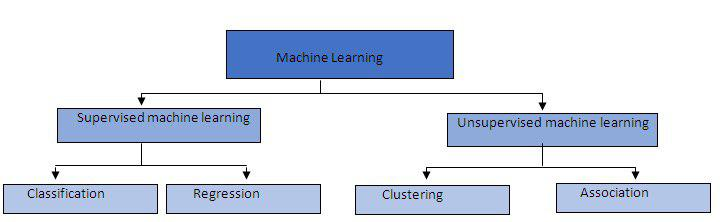
\includegraphics[keepaspectratio=true, width=0.9\textwidth]{disciplines.jpg}
    \caption{Distinction between supervised and unsupervised learning}
    \label{fig:class}
\end{figure}

The main difference between \textbf{classification} and \textbf{regression} is that when using classification, the result is \textbf{categorical}, whereas regression returns \textbf{numerical} results. 

\textbf{Clustering} is similar to classificiation. However, while classification algorithms sort the given data into given groups, clustering algorithms determine these groups \textbf{by themself}. This means, you can give a clustering algorithm a seemingly random dataset and the algorithm finds some kind of structure in it.

\newpage

\section{Data Quality}

Data is categorized into \textbf{numerical} and \textbf{categorical} data. 

\begin{figure}[htb!]
    \centering
    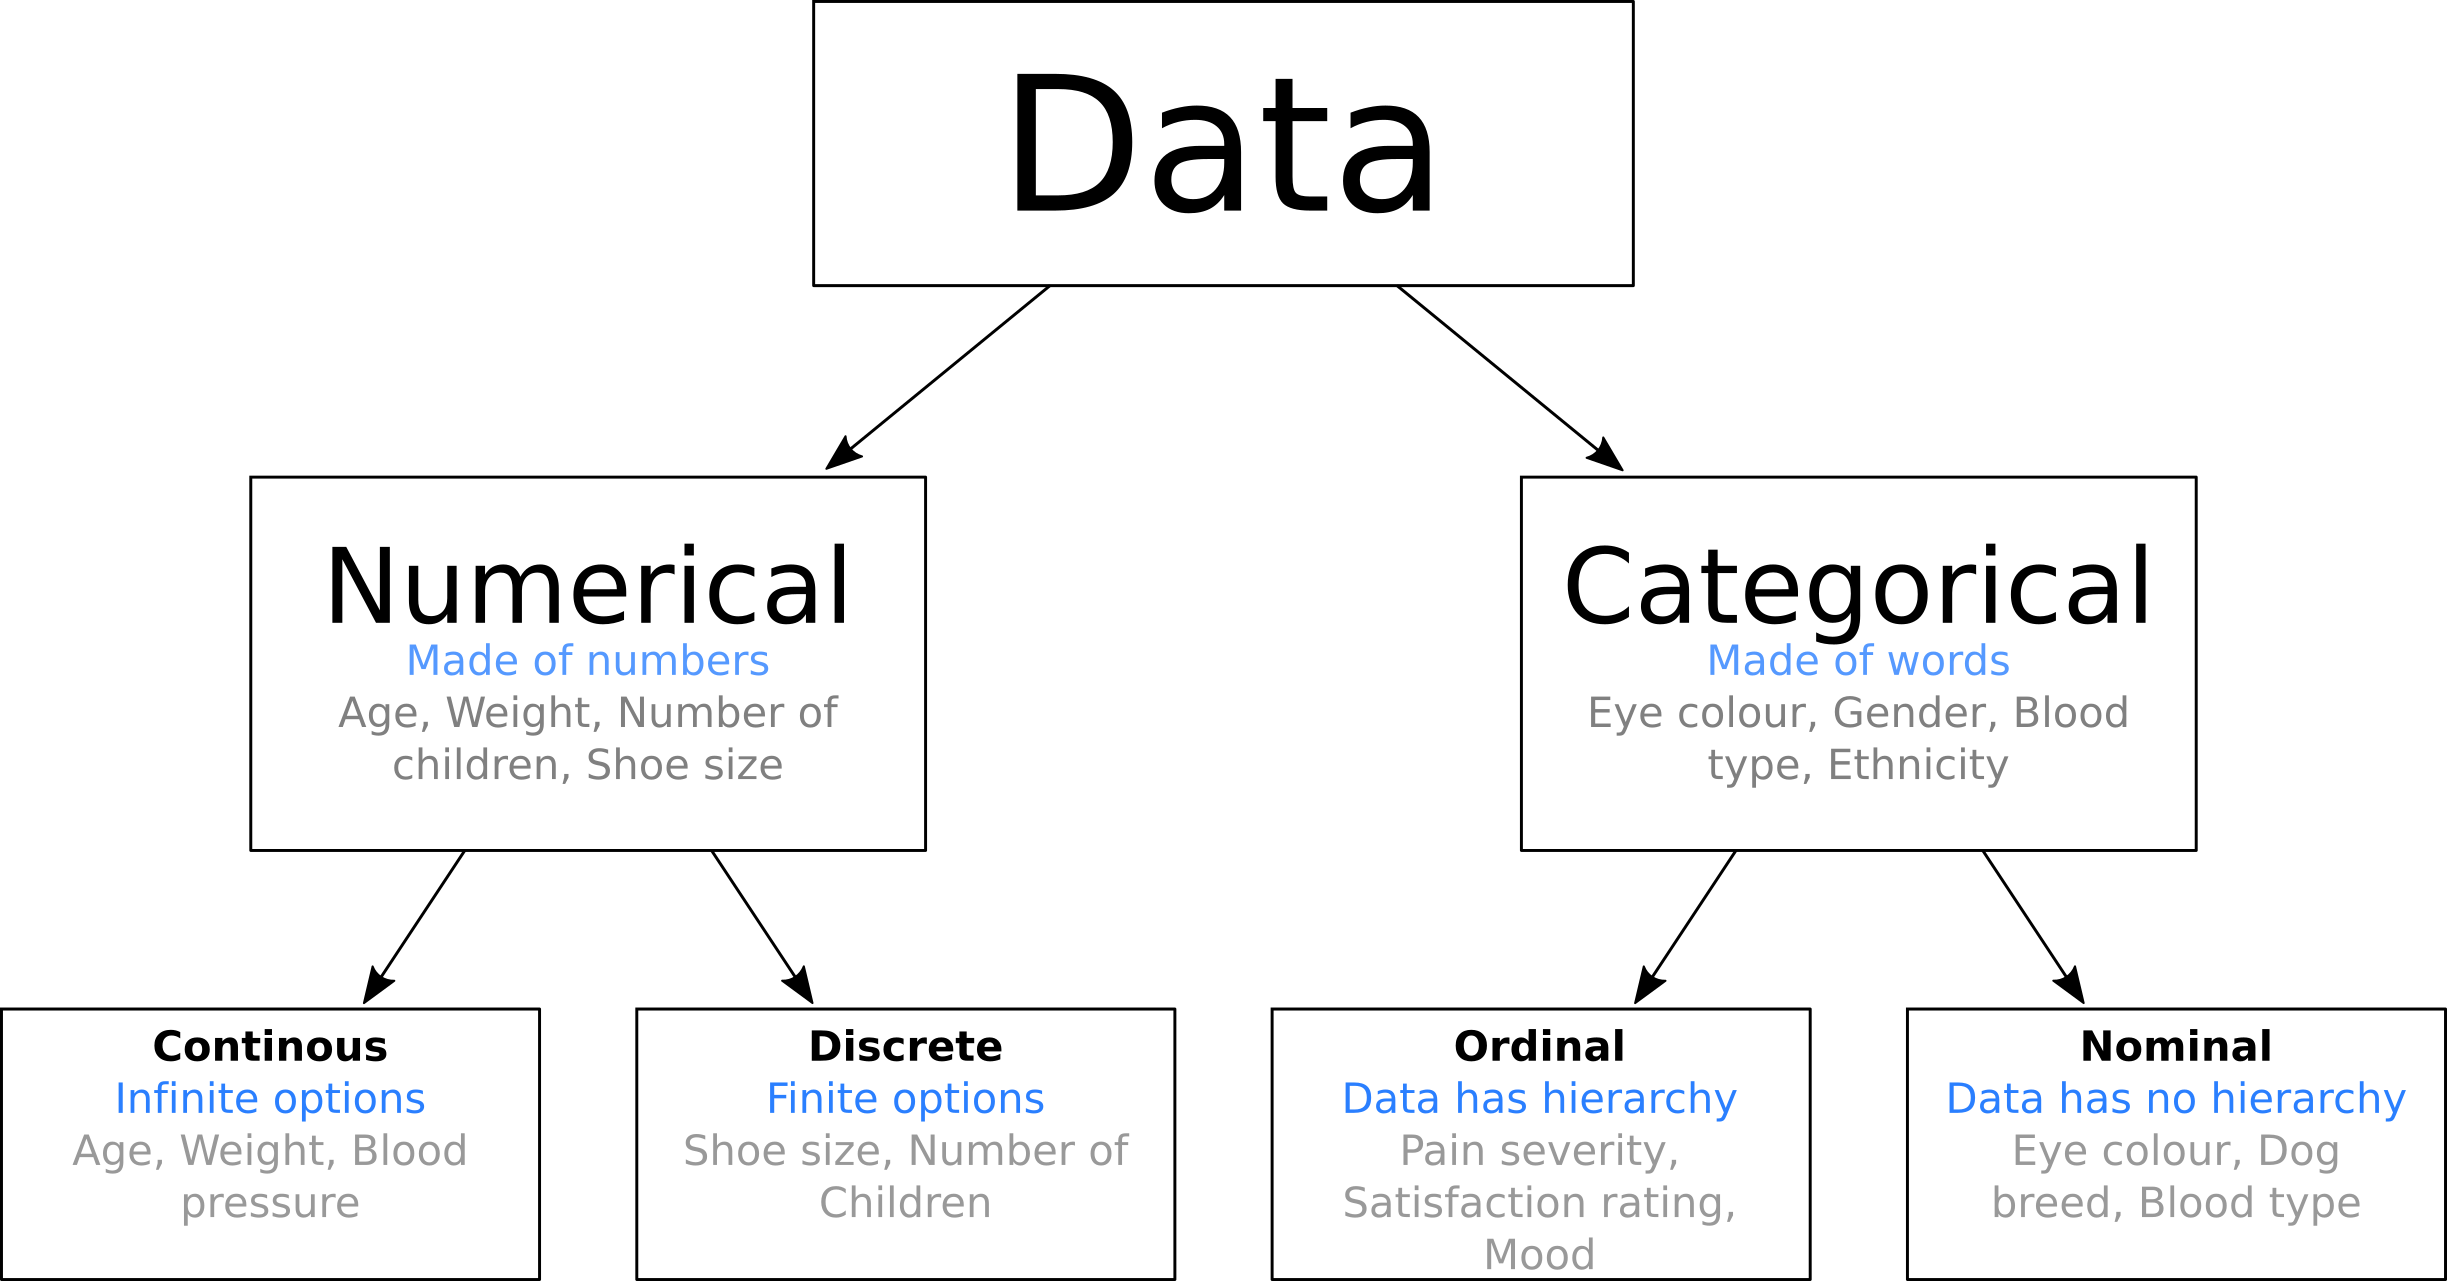
\includegraphics[keepaspectratio=true, width=0.9\textwidth]{data_classification.png}
    \caption{Classification of Data}
    \label{fig:data_classification}
\end{figure}

Before any machine learning can take place, the quality of the given data has to be assessed and in some cases improved. Because every prediction made by machine learning algorithms is shit if the data quality is shit.

There are many reasons why the data quality could be poor:

\begin{itemize}
    \item Ill-designed, inadequate or inconsistent data formats
    \item Programming errors or technical issues (e.g. sensor outage)
    \item Data decay (e.g. outdated e-mail addresses)
    \item Poorly designed data entry forms (e.g. data fields without verification)
    \item Human errors in data export or data pre-processing
    \item Deliberate errors and false information (e.g. due to privacy concerns everybody is called Hans Muster and lives at Musterstrasse 123)
\end{itemize}

\subsection{Data Quality Assessment}

Before even starting to assess the data-quality, it is seldomly a bad idea to \textbf{clean} the data first.

\begin{enumerate}
    \item Identify and remove duplicates
    \item Replace null-values (do not delete them because that might falsify the mean and median of the data)
    \item Make data formats more machine-friendly (so-called \textit{data-wrangling} e.g. store the gender as boolean)
\end{enumerate}

\newpage

If you change anything from the original data set, you should always

\begin{itemize}
    \item Document all the changes
    \item Use a SVN (e.g. git)
    \item Let the data provider know that his data quality is shit (maybe they'll improve in the future)
    \item Investigate the origins of the poor data quality
\end{itemize}

\subsection{Approaches to Data Quality Assessment}

\begin{description}
    \item[Identify data sources and their trustworthiness]
    \item[Interpret statical key figures: ] See following sections
    \item[Visualize selected portions of the data: ] e.g. with Pair Plots (See Abb. \ref{fig:pair_plots} )
    \item[Manually check data ranges] Negative Salaries, People more than 200 years old...
    \item[Validate plausibility of attribute correlation: ] e.g. are mileage and number of seats in a core correlated? Can one of the columns be removed for redundancy?
    \item[Measure data redundancy: ] Can certain columns be removed due to not adding any real value to the data
    \item[Check for anomalies in syntax and semantics: ] Outliers can really distort a dataset and render the whole algorithm useless. Can be prevented by e.g. normalization of the data or removal of the outlier
    \item[Replace NULL Values and remove duplicate values]
\end{description}

There are different ways to cope with NULL variables, but they have to be addressed, as most machine learning algorithms do not play well with them. 

\begin{itemize}
    \item Delete all rows with NULL values \\
        Might be the easiest way if you have loads of data
    \item Fill in the missing values manually (e.g. from other sources) \\
        Might be the hardest way if you have loads of data
    \item Fill in a global constant like N/A, UNKNOWN
    \item Use a measure for central tendency \\
        e.g. take the mean if your data is symmetric or take the median if its skewed
    \item Use a measure for central tendency per class \\
        e.g. take different values for healthy and sick people
    \item Use e.g Regression to 'guess' the missing values
\end{itemize}

\begin{figure}[htb!]
    \centering
    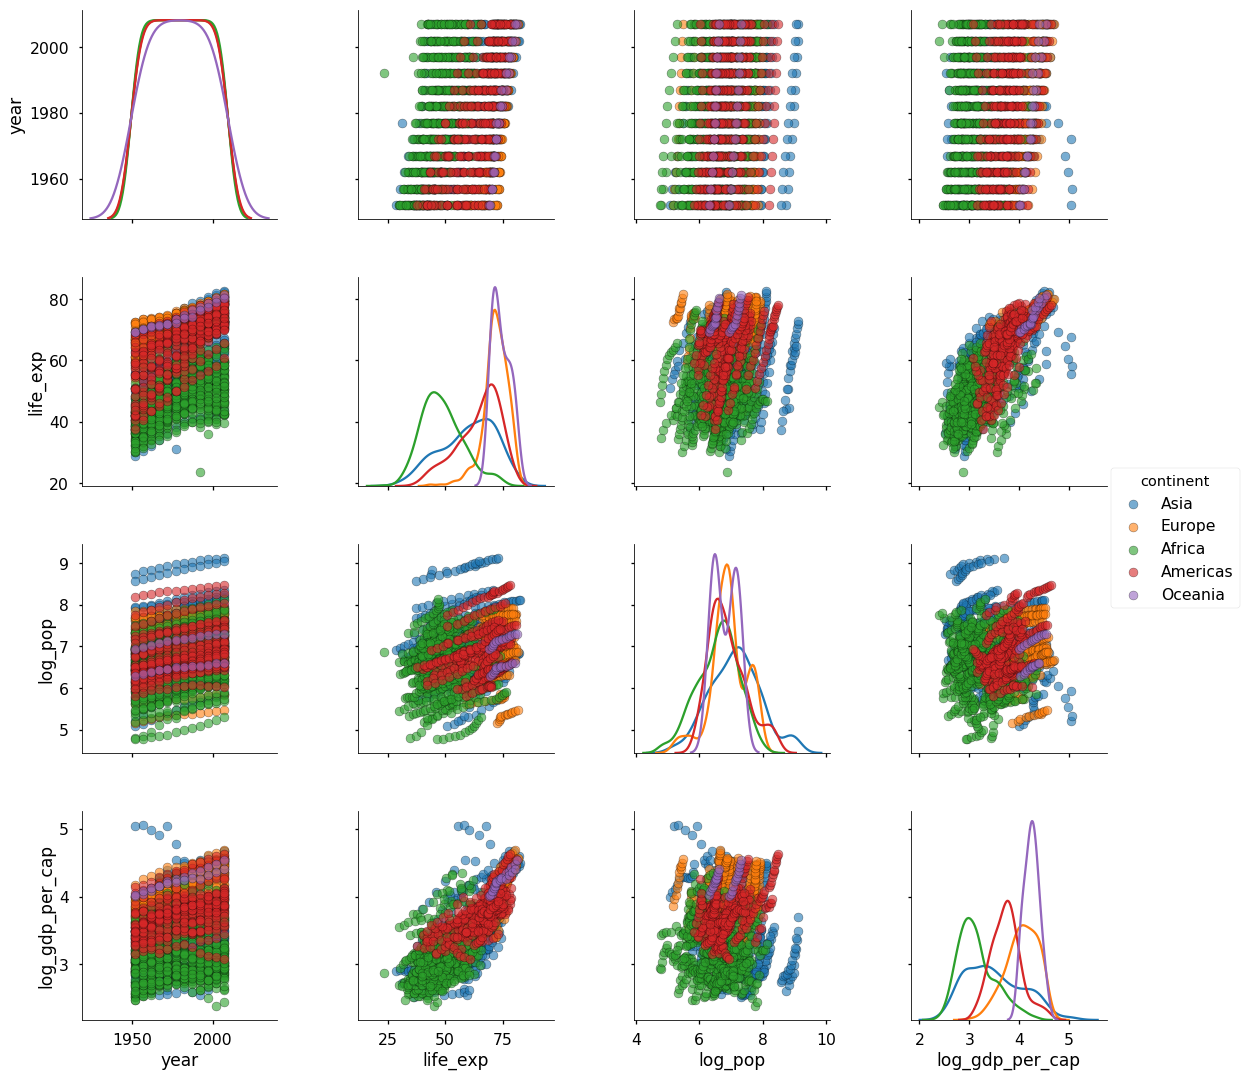
\includegraphics[keepaspectratio=true, width=0.4\textheight]{pair_plots.png}
    \caption{Visualisation of Data with Pair Plots}
    \label{fig:pair_plots}
\end{figure}

\newpage

\subsection{Statistical Key Figures}

These figures can give you a rough overview about the whereabouts of your data-magnitude.

\subsubsection{Central Tendency}

\textbf{Mean} \\

This is the averge in a set of numeric data. You add all data and divide it by the number of data points

\[ \scalebox{1.5}{
        $\mu_{x}=\frac{1}{n} \sum^{n}_{i=1} x_{i}$
}\]

\vspace{10px}

\noindent \textbf{Mode} \\

This is the value that occurs the most in a given set of data

\vspace{10px}

\noindent \textbf{Median} \\

This is the middlemost value of a sorted set of data. In contrast to the Mean, the Median can give information concerning the distribution of the data.

Given a dataset of $1, 2, 3, 4, 5$, the median and mean are both $3$. However, if we have $1, 2, 3, 1000, 10000$, the mean is $2201.2$ whereas the mean is still $3$ 

\newpage

\subsubsection{Skewdness}

All of these values can give information concerning the datas \textbf{skewness}

\begin{figure}[htb!]
    \centering
    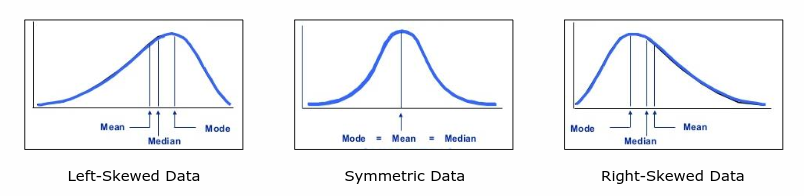
\includegraphics[keepaspectratio=true, width=0.9\textwidth]{skewness.png}
    \caption{Skewness of data}
    \label{fig:skewness}
\end{figure}

\noindent    
$Mean - Mode > 0 \rightarrow$ Negative skewness / Left-skewed data \\
$Mean - Mode = 0 \rightarrow$ Symmetric Data \\
$Mean - Mode > 0 \rightarrow$ Positive skewness / Right-skewed data

\vspace{10px}

\subsubsection{Quartile \& Interquartile Range (IQR)}

The three quartiles divide your data into four equal-sized, cnsecutive subsets.

To calculate $Q1$, take the median of your data and then again the madian of the left half of the data.

\begin{figure}[htb!]
    \centering
    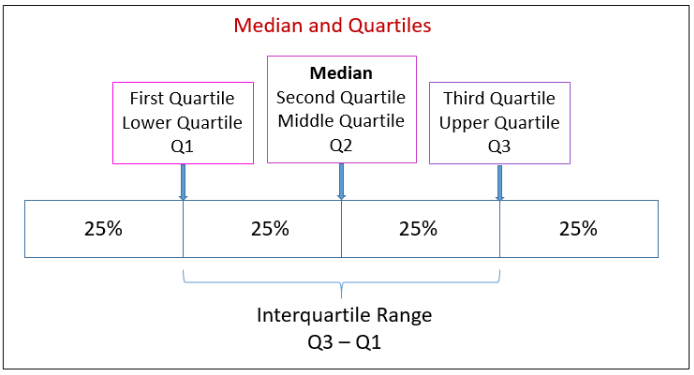
\includegraphics[keepaspectratio=true, width=0.9\textwidth]{iqr.png}
    \caption{Quartiles of a dataset}
    \label{fig:iqr}
\end{figure}

\newpage
 
\subsubsection{Five Number Summary}

With this method, you can get a pretty good overview of your data. The \textbf{Five Number Summary} of a dataset consists of:

\begin{itemize}
    \item Median Q2
    \item Quartiles Q1 and Q2
    \item Smallest individual Value
    \item Largest individual Value
\end{itemize}

\begin{minipage}{0.45\textwidth}
    \begin{lstlisting}[caption={Five Number Summary in Python}]
    import numpy as np
    import panas as pd

    s = pd.Series(np.random.rand(100))
    s.describe()
    \end{lstlisting}
\end{minipage}\hfill
\begin{minipage}{0.45\textwidth}
    \begin{lstlisting}[caption={Output}]
    mean       0.524559
    std        0.285565
    min        0.003933
    25%        0.298367
    50%        0.530632
    75%        0.765907
    max        0.993293
    dtype: float64
    \end{lstlisting}
\end{minipage}

\subsubsection{Boxplot}

\begin{wrapfigure}[14]{R}{0.5\textwidth}
    \centering
    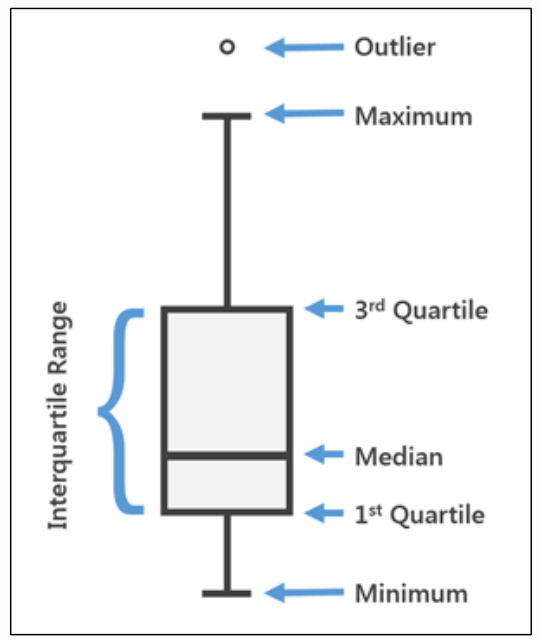
\includegraphics[keepaspectratio=true,height=14\baselineskip]{boxplot.png}
    \caption{Boxplot}
    \label{fig:boxplot}
\end{wrapfigure}

This plot is a \textbf{visual representation of the five number summary} and can also give information on potential outliers. 

Values $1.5 \cdot IQR$ above the 3rd or below the 1st Quartile can be considered outliers and are displayed with small circles. 

\subsubsection{Variance}
The variance shows \textbf{how much the values are spread on average}. This is measured by squaring the sum of all deviations from the mean

\[ \scalebox{1.5}{
        $\dfrac{1}{1-n} \sum^{n}_{i=1}(x_{i} - \mu x)^2$
}\]

The standard deviation is calculated as $\sqrt{variance}$

\newpage

\subsubsection{Covariance}
The covariance is used to determine whether two variables are \textbf{connected} to each other. 

If both variables are on the same side of the mean, the variance is \textbf{positive}, the variables are probably connected. Meaning if the value of one variable is rising, the other one will most likely rise as well. 

If one is above and one is below the mean, the variance is \textbf{negative}, the variables are most likely \textbf{inversely connected} to each other. Meaning if the value of one variable is rising, the other is most likely falling.

If the variables are \textbf{independent} from each other, the covariance is zero, as they both cancel each other out.

\[\scalebox{1.5}{
        $Cov(x,y)\dfrac{1}{1-n} \sum^{n}_{i=1}(x_{i} - \mu x)(y_{i} - \mu y)$
}\]

The \textbf{covariance matrix} shows the covariance from all $X$ with all $Y$. As $Cov(x,x) = Var(x)$, the covariance matrix has the variance of $X$ in its diagonal


\subsubsection{Pearson Correlation}
Both the covariance and the variance are connected to the scale of the dataset, so the covariance of $X=[1,2,3,4,5] / Y=[6,7,8,9,10]$ is 2.5, whereas the covariance of $X=[1000,2000,3000,4000,5000] / Y=[6000,7000,8000,9000,10000]$ is 2'500'000'000. However, the Perason Correlation is 1 in both examples.

\[\scalebox{1.5}{
        $\rho(X,Y)=\dfrac{Cov(X,Y)}{\sigma_{x} \sigma_{y}}$
}\]

The Pearson Correlation is always between 1 and -1. 

\noindent 1 means the data is perfectly correlated, whereas -1 means that the data is perfectly incorrelated

\subsection{Normalization}
It is immensely important that all data is normalized before we run a machine learning algorithm over it. Considering the data in figure \ref{fig:vector_space_modefig}, 'Mileage' and 'Price' are in a completely different scale. If the mileage of the first shown car goes up 500 miles, it's not really a big deal. However, a price increase by 500 would double the car's price.

Such differently scaled data can (and will) falsify the result of every machine learning algorithm you could find. Therefore, \textbf{normalization is really important}.

\vspace{10px}

\noindent There are two popular normalization approaches: The Min-Max and the Z-Score normalization. 

\vspace{10px}

\noindent \textbf{Min-Max normalization}

\noindent All data is condensed to a value between 0 and 1. The smallest value becomes 0 and the largest one becomes 1.

\[\scalebox{1.5}{
        $x \rightarrow \dfrac{x - min_{x}}{max_{x}-min_{x}}$
}\]

\newpage

\noindent \textbf{Z-Score Normalization}

\noindent The dataset is transformed in such a way, that the mean becomes 0 (so-called \textit{mean-centering}) and the standard deviation is 1

\[\scalebox{1.5}{
        $x \rightarrow \dfrac{x - \mu_{x}}{\sigma_{x}}$
}\]

\section{Geometry of Data}

\subsection{Feature Engineering}

Sometimes, data has to be modified to be better accessible/processable for machine learning algorithms. These algorithmus can work the best with simple numbers, so that's the data we should be striving for:

\begin{figure}[htb!]
    \centering
    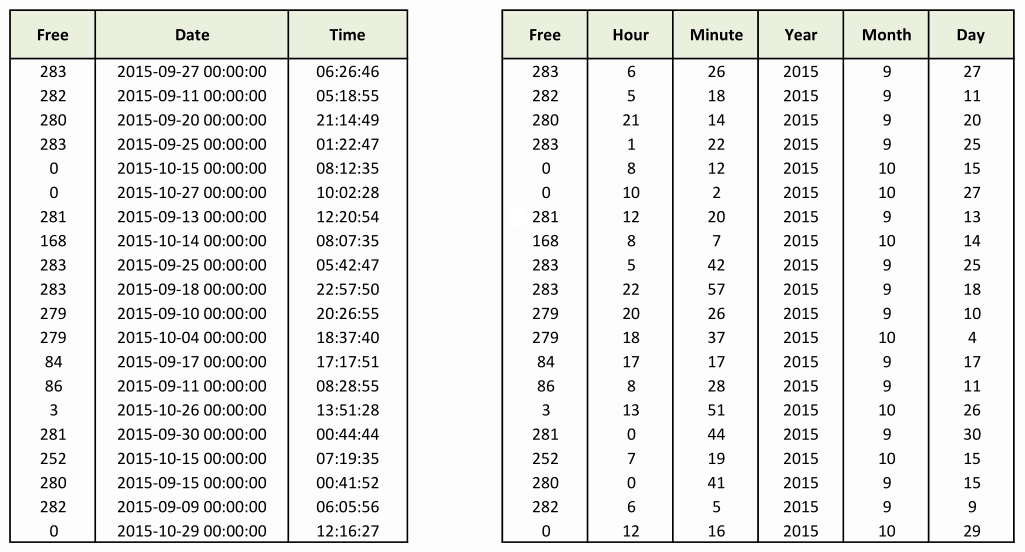
\includegraphics[keepaspectratio=true, width=\linewidth]{feature_engineering.png}
    \caption{Turn 'complicated' data into easier data for better results}
    \label{fig:feature_engineering}
\end{figure}

\subsection{Vector Space Model}

As described before, machine learning algorithms work best with \textbf{numeric} data. However, the real world isn't that easy and mostly throws categorical data at you. Therefore, you have to convert categorical data to numerical data. 

\begin{figure}[htb!]
    \centering
    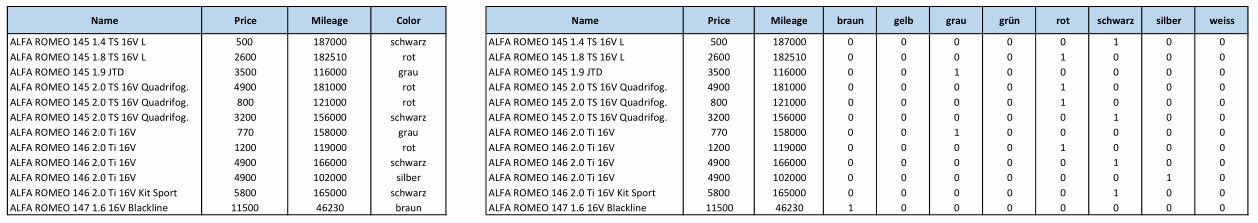
\includegraphics[keepaspectratio=true, width=\linewidth]{vector_space_model.png}
    \caption{Turn categorical data into numerical data with the vector space model}
    \label{fig:vector_space_modefig}
\end{figure}

This transformed data can also be visualized in a coordinate system and we can do math with it.

\begin{figure}[htb!]
    \centering
    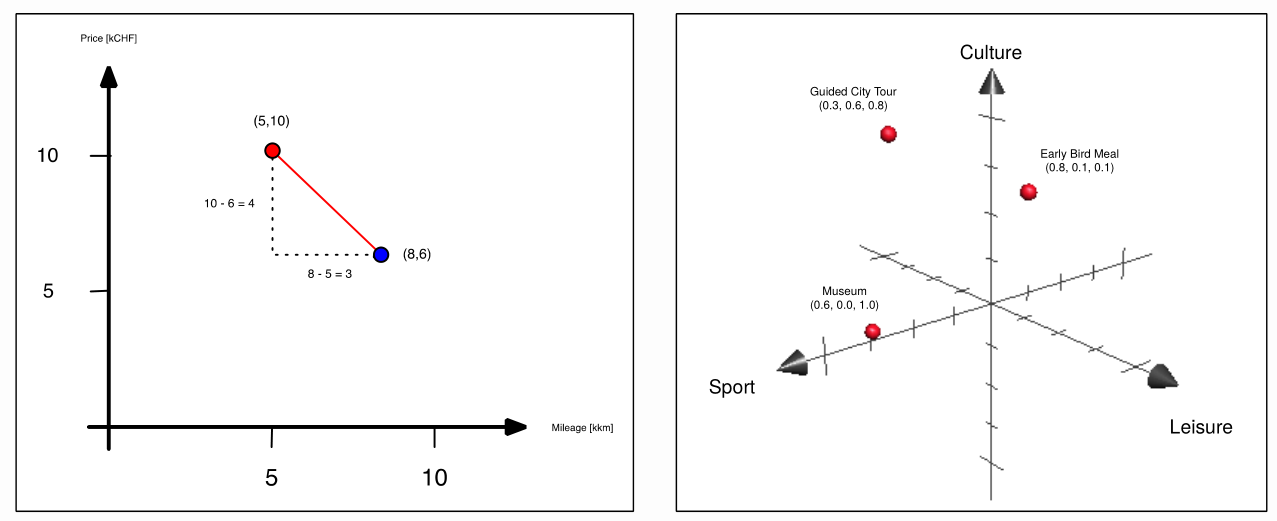
\includegraphics[keepaspectratio=true, width=\linewidth]{geometric_interpretation.png}
    \caption{Transformed into vector space, data points can be interpreted as geometric points}
    \label{fig:geometric_intepretation}
\end{figure}

\subsection{Similarity of Data}

The math we want to do is not even overly complicated: We just want to measure the distance between different points. Because \textbf{the smaller the distance between two points, the more similar they are}. 

\subsubsection{Euclidean Distance}

The distance between two points is most easily calculated using the \textbf{euclidean distance}:

\[\scalebox{1.5}{
        $dist(X,Y)= \sqrt{\sum^{n}_{i=1}(x_{i}-y{i})^2} $
}\]

So the distance between the points $(5/10)$ and $(8/6)$ can be calculated as

\begin{align*}
    \sqrt{(5-8)^2 + (10-6)^2} \\
    \sqrt{-3^2 + 4^2} \\
    \sqrt{9+16} \\ 
    \sqrt{25} = 5
\end{align*}

\newpage

\subsubsection{Cosine Similarity}

\begin{wrapfigure}[14]{R}{0.5\textwidth}
    \centering
    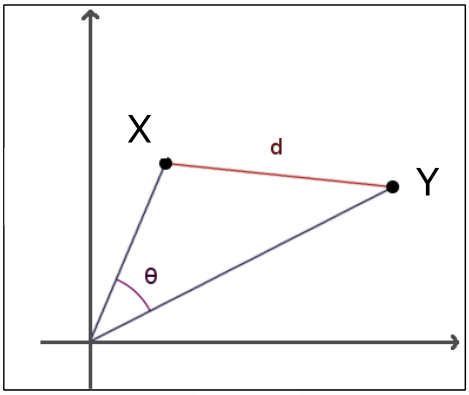
\includegraphics[keepaspectratio=true,height=14\baselineskip]{cosine_similarity.png}
    \caption{Cosine Similarity}
    \label{fig:cosine_similarity}
\end{wrapfigure}

If you want to to compare two points that appear to be on a line (Pearson Correlation close to 1), but the euclidean distance is high, then the cosine similarity is probably pretty low. 

The cosine similarity looks at the \textbf{angle} between point A and point B. However, it does also take the euclidean distance into consideration.

\vspace{10px}

The cosine similarity is essentially just the scalar product of the two points.

\vspace{10px}

\[\scalebox{1.5}{
    $sim(X,Y) = \dfrac{\sum^{n}_{i=i}{x_{i} y_{i}}}{\sqrt{\sum^{n}_{i=i}{x_{i}}^2\sqrt{\sum^{n}_{i=i}{y_{i}}^2}}}$
}\]
\[\scalebox{1.5}{
    $dist(X,Y) = 1 - sim(X,Y)$
}\]

\subsubsection{Levenshtein / Edit Distance for Strings}

Count the minimal number of changes necessary to turn one string into another:
\begin{itemize}
\item count +1 when deleting a character [d]
\item count +1 when adding a character [a]
\item count +2 when changing a character [c]
\end{itemize}

\begin{figure}[htb!]
    \centering
    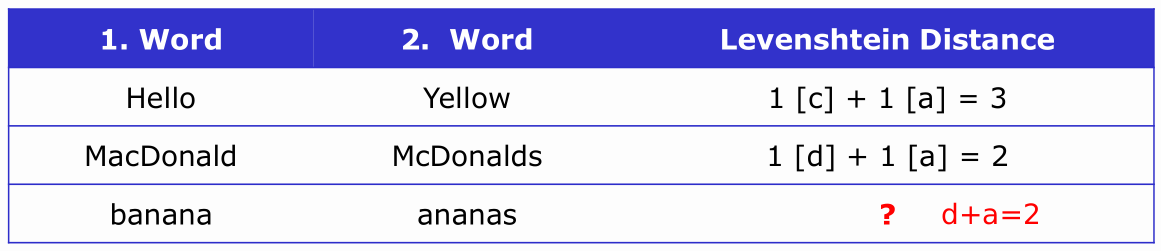
\includegraphics[keepaspectratio=true, width=\linewidth]{levenshtein.png}
    \caption{Examples for Levenshtein Distance}
    \label{fig:levenshtein}
\end{figure}

\end{document}

